\chapter{\ifenglish Background Knowledge and Theory\else ทฤษฎีที่เกี่ยวข้อง\fi}

การทำโครงงาน เริ่มต้นด้วยการศึกษาค้นคว้า ทฤษฎีที่เกี่ยวข้อง หรือ งานวิจัย/โครงงาน ที่เคยมีผู้นำเสนอไว้แล้ว ซึ่งเนื้อหาในบทนี้ก็จะเกี่ยวกับการอธิบายถึงสิ่งที่เกี่ยวข้องกับโครงงาน เพื่อให้ผู้อ่านเข้าใจเนื้อหาในบทถัดๆ ไปได้ง่ายขึ้น

\section{ตรรกศาสตร์คลุมเครือ (Fuzzy Logic)}
ตรรกศาสตร์คลุมเครือ เป็นแนวคิดเกี่ยวกับการวิเคราะห์เชิงตรรกะ แต่การวิเคราะห์ไม่ได้มีเพียง ถูกกับผิด หรือ 0 กับ 1 เนื่องจากเหตุการณ์ในความเป็นจริงสร้างความคลุมเครือในการวิเคราะห์ เช่น อุณหภูมิอากาศ 20 องศาเซลเซียสเป็นอากาศที่หนาวไปหรือไม่? หากนำคำถามนี้ไปให้ผู้วิเคราะห์ต่างที่อยู่อาศัยกัน จะได้คำตอบที่ไม่เหมือนกัน เนื่องจากการวิเคราะห์แนวนี้ไม่เหมาะกับการตอบเพียงใช่หรือไม่ การใช้ตรรกศาสตร์คลุมเครือ (Fuzzy Logic) มาใช้วิเคราะห์เหตุการณ์จึงจะได้คำตอบที่ดีกว่า แทนที่จะตอบเพียงแค่ ใช่หรือไม่ คำตอบที่ได้จะเป็นพจน์ของ ตัวแปรทางภาษา (Linguistic Variable) และความเป็นสมาชิก เช่นตัวแปรทางภาษาอุณหภูมิมีค่า หนาว 60\% อบอุ่น 15\% ร้อน 0\% (เพราะผู้วิเคราะห์อาจจะรู้สึกหนาวแต่ก็ไม่ได้หนาวเกินไปหรืออบอุ่นอยู่เล็กน้อย) จะเห็นว่าการบอกค่าเชิงตรรกะแบบฟัซซีสะท้อนความจริงได้ดีกว่าการตอบแบบเดิม

% \section{Second section}
% Section 2 text.

\subsection{ฟัซซีเซต (Fuzzy Set)}
เป็นเซตที่ขอบเขตไม่เด่นชัดหรือคลุมเครือโดยการบอกค่าเชิงตรรกะจะถูกสร้างเป็นฟัซซีเซตที่เราสามารถวัดระดับความเป็นสมาชิก (Membership Value) ของสมาชิกในเอกภพสัมพัทธ์ต่อฟัซซีเซตนั้นผ่านทางฟังก์ชันภาวะสมาชิก (Membership function) ซึ่งเป็นฟังก์ชันที่รับสมาชิกในเอกภพสัมพัทธ์แล้วส่งไปที่ช่วง [0,1] โดยจากตัวอย่างดังกล่าวจะสามารถสร้างเป็นฟัซซีเซ็ตได้เป็น เซ็ตของอากาศ เย็น, อบอุ่น, ร้อน โดยให้อุณหภูมิเป็นสมาชิกของเซ็ตซึ่งสมาชิกแต่ละตัวสามารถเป็นสมาชิกของทุกเซ็ตได้ เช่น อุณหภูมิ 20 องศาเซลเซียส มีระดับความเป็นสมาชิกในฟัซซีเซตอากาศเย็น 0.6, อบอุ่น 0.15, ร้อน 0
\begin{figure}[ht]
    \centering
    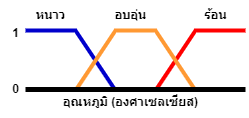
\includegraphics[scale=0.7]{images/fuzzy_set.png}
    \caption{ฟัซซีเซต หนาว,อบอุ่น,ร้อน และฟังก์ชันภาวะสมาชิก}
    \label{fig:4}
\end{figure}

\subsection{ระบบประมวลผลตรรกศาสตร์คลุมเครือ (Fuzzy Logic System)}
เป็นการนำเอาความสามารถของตรรกศาสตร์คลุมเครือมาสร้างเป็นระบบประมวลผลแบบตรรกศาสตร์คลุมเครือซึ่งเป็นการเลียนแบบการคิด การหาเหตุผล การตัดสินใจและการกระทำของมนุษย์ โดยจะมีส่วนประกอบสำคัญ 4 ส่วนคือ 1. การแปลงข้อมูลขาเข้าเป็นฟัซซี (Fuzzification), 2. กฏ (Fuzzy Rules), 3. การอนุมานหรือการตีความ (Inference), 4. การแปลงข้อมูลฟัซซีเป็นตัวเลข (Defuzzification)
ซึ่งจะมีตัวอย่างการทำงานเมื่อใช้ระบบประมวลผลตรรกศาสตร์คลุมเครือดังภาพรวมนี้
\begin{figure}[ht]
    \centering
    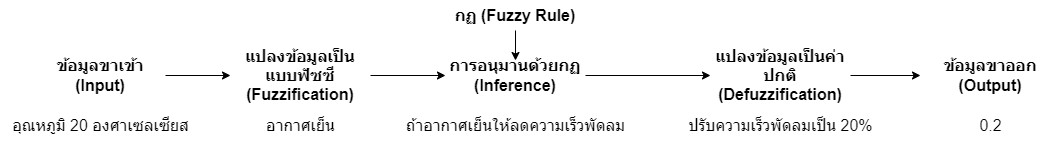
\includegraphics[scale=0.375]{images/ex_fis.png}
    \caption{ตัวอย่างการทำงานของระบบประมวลผลตรรกศาสตร์คลุมเครือ}
    \label{fig:5}
\end{figure}

โดยในงานนี้เราใช้ระบบฟัซซีแบบ Mamdani

\subsubsection{การแปลงข้อมูลขาเข้าเป็นฟัซซี (Fuzzification)}
เป็นการแปลงข้อมูลอินพุตทั่วไปที่เป็นตัวเลข (Crisp Set) ไปเป็นข้อมูลในรูปแบบฟัซซีเซต หรือที่เรียกว่าตัวแปรทางภาษา (Linguistic Variable) โดยจะสร้างฟังก์ชันภาวะสมาชิกซึ่งขึ้นอยู่กับลักษณะของข้อมูลขาเข้าและความสำคัญต่อข้อมูลเอาท์พุต
\begin{equation} \mu_A(x) = \begin{cases}
0 & \text{if } x \leq a \\
\frac{x-a}{b-a} & \text{if } a < x < b \\
\frac{c-x}{c-b} & \text{if } b \leq x < c \\
0 & \text{if } x \geq c \\
\end{cases} \end{equation}
\begin{figure}[ht]
    \centering
    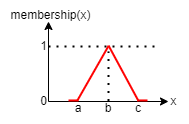
\includegraphics[scale=0.7]{images/ex_memship.png}
    \caption{ตัวอย่างกราฟฟังก์ชันภาวะสมาชิก Triangular function}
    \label{fig:6}
\end{figure}

\subsubsection{กฏฟัซซี (Fuzzy Rules)}
เป็นส่วนของการกำหนดวิธีการควบคุมซึ่งได้มาจากผู้เชี่ยวชาญหรือการปรับแต่งทดลองขึ้นเองโดยจะอยู่ในรูปแบบของชุดข้อมูลแบบกฏของภาษา ซึ่งกฏฟัซซีแบบที่นิยมใช้มากและใช้ในงานนี้เป็นกฏฟัซซีแบบ ถ้า-แล้ว (If-then rule)
โดยในงานนี้ได้ใช้วิธีการของ Mamdani หากมีอินพุต \(X_{1},X_{2},...,X_{n}\) และพจน์ภาษา \(T(x_{i})\) ของตัวแปรทางภาษา \(x_{i}\) ในเซตสากล \(X_{i}\) สำหรับ \(1 \le i \le n\) ในขณะเดียวกัน \(Y\) ก็ถูกนิยามด้วยตัวแปรทางภาษา และพจน์ภาษา \(T(y)\) ของตัวแปรทางภาษา y ในเซตสากล \(Y\)
\[ IF\; x_{1}\; is\; A^{(1)}\; and\; x_{2}\; is\; A^{(2)}\; and\; ... \; and\; x_{n}\; is\; A^{(n)}\; THEN\; y\; is\; B \]
โดยที่ \(A^{(1)},A^{(2)},...,A^{(n)}\) เป็นพจน์ในภาษา \(T(x_{i})\) และ B เป็นพจน์ในภาษา \(T(y)\)

\subsubsection{การอนุมานหรือการตีความ (Inference)}
เป็นส่วนของการประมวลผลจะมีการตีความตามเงื่อนไขที่กำหนดไว้ หรือก็คือตีความผ่านกฏฟัซซี ซึ่งจากกฏฟัซซีดังกล่าวจะประกอบด้วยกันสองส่วนคือ ส่วนที่เกิดขึ้นก่อน (If Part) และผลที่ตามมา (Then part) โดยที่อินพุตและเอาท์พุตนั้นอาจมีหลายตัวก็ได้ขึ้นอยู่กับการออกแบบ ผลที่ตามมาของแต่ละกฏจะถูกรวมกันด้วยวิธีทางตรรกศาสตร์เพื่อให้ได้ค่าเอาท์พุตเพียงค่าเดียว

โดยจะเริ่มจากการหาระดับความเข้ากันได้ของแต่ละอินพุต \((x_{i}, i \in \{1,2,...,n\})\) กับพจน์ภาษาในกฏนั้น และเนื่องจากลักษณะของส่วนที่เกิดขึ้นก่อน (If Part) ของกฏต้องการให้ทุกอินพุตเป็นไปตามพจน์ภาษา ดังนั้นค่าความเป็นสมาชิกของแต่ละอินพุตในแต่ละพจน์ภาษาจะถูกรวมกันในลักษณะของตัวเชื่อม conjunction นั่นคือที่กฏ j
\begin{equation}
\alpha_{j} = min\{A^{(1)}_{i1,j}(x_{1}), A^{(2)}_{i2,j}(x_{2}), ..., A^{(n)}_{in,j}(X_{n})\}
\end{equation}
และเอาต์พุตของกฏ j เป็นฟัซซีเซตที่เกิดจากการตัด (cut off) พจน์ภาษา \(B_{i,j}\) ด้วย \(\alpha_{j}\) หรือ
\begin{equation}
OUT^{(j)}_{x_{1},x_{2},...,x_{n}} (y) = min(A^{(1)}_{i1,j}(x_{1}), A^{(2)}_{i2,j}(x_{2}),...,A^{(n)}_{in,j}(x_{n}),B_{i,j}(y))
\end{equation}
และเมื่อได้เอาต์พุตของแต่ละกฏแล้ว ฟัซซีเอาต์พุตจากทุกกฏจะถูกรวมกันโดยการหาฟัซซียูเนียนมาตรฐาน (ซึ่งจะได้ฟัซซีเอาต์พุตรวม (OUT)) สมมติให้มีกฏทั้งหมด k กฏ จะได้ OUT เป็น
\begin{equation}
OUT_{x_{1},x_{2},...,x_{n}} (y) = max_{j \in \{1,2,...,k\}}\; min(A^{(1)}_{i1,j}(x_{1}), A^{(2)}_{i2,j}(x_{2}),...,A^{(n)}_{in,j}(x_{n}),B_{i,j}(y))
\end{equation}
ตัวอย่าง สมมติให้ระบบมีกฏ 2 กฏ โดยที่แต่ละกฏจะมีอินพุต 2 อินพุต และแต่ละอินพุตในแต่ละกฏมีพจน์ภาษาดังรูป โดยที่มีกฏดังนี้คือ
\[R1:\; IF\; x_{1}\; is\; L_{1}\; and\; x_{2}\; is\; H_{2},\; THEN\; y\; is\; L \]
\[R2:\; IF\; x_{1}\; is\; M_{1}\; and\; x_{2}\; is\; M_{2},\; THEN\; y\; is\; H \]
ถ้ากำหนดให้ \(x_{1}\) มีค่าเท่ากับ 2 และ \(x_{2}\) มีค่าเท่ากับ 5 จะได้ว่า
\[\alpha_{1} = min(L_{1}(x_{1}),H_{2}(x_{2})) = min (1,0.5) = 0.5\]
\[\alpha_{2} = min(M_{1}(x_{1}),H_{2}(x_{2})) = min (0,0.5) = 0\]ฟัซซีเอาต์พุตของกฏที่ 1 และ 2 และฟัซซีเอาต์พุตรวม (OUT) แสดงในรูปดังนี้
\begin{figure}[ht]
    \centering
    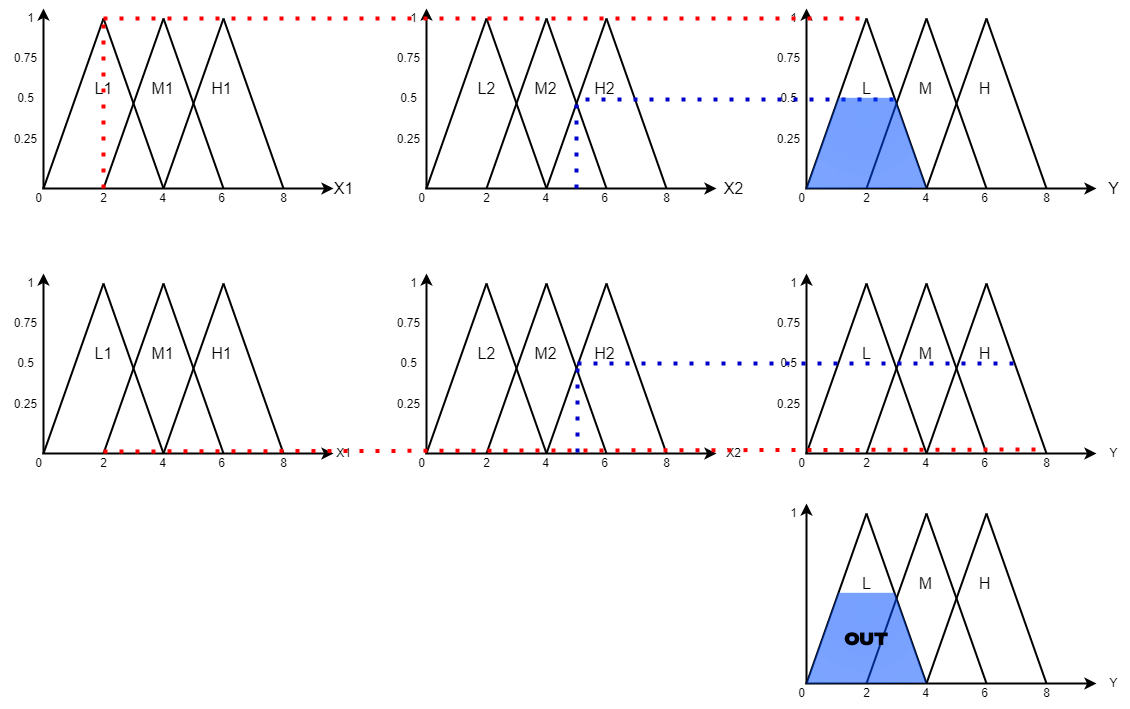
\includegraphics[scale=0.3]{images/ex_inference.png}
    \caption{ตัวอย่างการอนุมาน}
    \label{fig:7}
\end{figure}

\subsubsection{การแปลงข้อมูลฟัซซีเป็นค่าปกติ (Defuzzification)}
เนื่องจากผลลัพธ์ที่ได้จากการตีความนั้นยังอยู่ในรูปแบบของฟัซซี ในส่วนนี้เป็นการทำการแปลงข้อมูลที่อยู่ในรูปแบบฟัซซีเป็นข้อมูลที่เป็นตัวเลข (Crisp set) ด้วยวิธีทางคณิตศาสตร์ เช่น Center of Area (Centroid) เพื่อนำค่าที่ได้มาใช้ในการตัดสินใจและนำไปควบคุมระบบได้

วิธีแปลงโดยการหา Centroid จะหาค่าเอาต์พุตจากจุดศูนย์กลางของพื้นที่กราฟได้ดังสมการนี้
\begin{equation}
  de_y = \frac{\int B(z)\cdot zdz}{\int B(z)dz}
\end{equation}

โดย \(B(z)\) คือ ค่าความเป็นสมาชิก (Membership Value) ของตำแหน่ง \(z\)

\section{การหาค่าที่เหมาะสมที่สุดโดยกลุ่มของอนุภาค (Particle Swarm Optimization (PSO))}
การหาค่าที่เหมาะสมที่สุดโดยกลุ่มของอนุภาค เป็นอัลกอริทึมการค้นหาที่ขึ้นกับประชากร ซึ่งเป็นการจำลองพฤติกรรมเชิงสังคมของฝูงนก ท่าทางของฝูงนกเชิงภูมิศาสตร์ที่คาดเดาไม่ได้ โดยที่มีจุดประสงค์ในการค้นพบรูปแบบที่ควบคุมความสามารถของนกในการบินพร้อมกันและสามารถเปลี่ยนทิศทางได้อย่างกะทันหัน โดยการรวมกลุ่มกันใหม่ในลักษณะที่เหมาะสมที่สุด ทำให้เกิดอัลกอริทึมสำหรับการจัดระเบียบกลุ่มของอนุภาค ที่ง่ายและมีประสิทธิภาพ

\subsection{อนุภาค (Particle)}
อนุภาค 1 อนุภาค คือคำตอบที่เป็นไปได้ของปัญหาการหาค่าที่เหมาะสม โดยอนุภาคจะบินในปริภูมิการค้นหาหลายมิติ การเปลี่ยนแปลงของอนุภาคในกลุ่มนั้นมีอิทธิพลมาจากประสบการณ์ หรือความรู้ของเพื่อนบ้าน รูปร่างของเพื่อนบ้านมีหลายรูปแบบ และมีการสร้างอัลกอริทึมตามแต่ละรูปแบบ

\subsubsection{ทอพอโลยีแบบดาว (star topology)}
รูปแบบนี้ทำให้แต่ละอนุภาคสามารถติดต่อกับอนุภาคอื่นได้ทุกอนุภาค แต่ละอนุภาคจะสนใจอนุภาคที่ดีที่สุดในกลุ่ม และแต่ละอนุภาคจะเลียนแบบอนุภาคที่ดีที่สุดในกลุ่มนี้เอง โดยอัลกอริทึมที่จำลองสถานการณ์นี้คือ อัลกอริทึมดีที่สุดแบบรวม (global best)
\begin{figure}[ht]
    \centering
    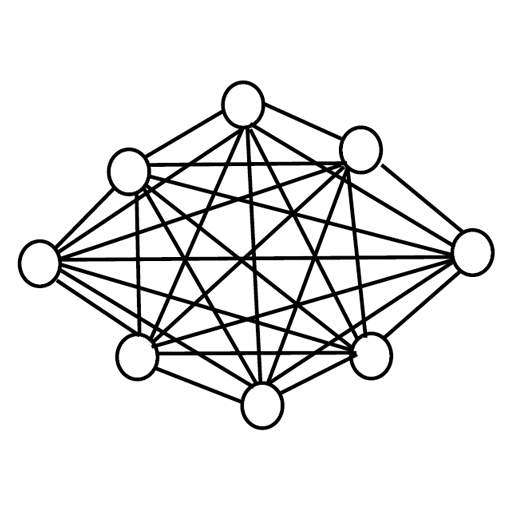
\includegraphics[scale=0.3]{images/star_topology.png}
    \caption{รูปแบบของเพื่อนบ้านสำหรับการจัดระเบียบกลุ่มของอนุภาค ทอพอโลยีแบบดาว}
    \label{fig:8}
\end{figure}

\subsubsection{ทอพอโลยีแบบวงแหวน (ring topology)}
รูปแบบนี้ทำให้แต่ละอนุภาคจะติดต่อได้กับเพื่อนบ้านที่ใกล้ที่สุด \(n\) อนุภาค ดังแสดงในรูป เมื่อ \(n=2\) ดังนั้นอนุภาคเคลื่อนที่ตามเพื่อนดีที่ในกลุ่มเพื่อนบ้านที่ติดต่อได้ ซึ่งอัลกอริทึมที่จำลองสถานการณ์นี้คือ อัลกอริทึมดีที่สุดแบบเฉพาะที่ (local best)
\begin{figure}[ht]
    \centering
    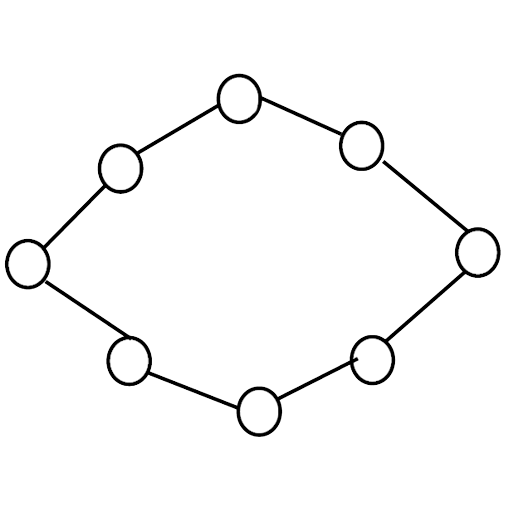
\includegraphics[scale=0.3]{images/ring_topology.png}
    \caption{รูปแบบของเพื่อนบ้านสำหรับการจัดระเบียบกลุ่มของอนุภาค ทอพอโลยีแบบวงแหวน}
    \label{fig:9}
\end{figure}

\subsection{อัลกอริทึมสำหรับการจัดระเบียบกลุ่มของอนุภาค}
อนุภาคจะบินอยู่ในปริภูมิการค้นหาหลายมิติ โดยที่ตำแหน่งของอนุภาคจะเปลี่ยนไปตามประสบการณ์ของตัวอนุภาคเอง หรือของเพื่อนบ้าน ให้ \(x_{i}(t)\) เป็นตำแหน่งของอนุภาค \(P_{i}\) ในปริภูมิไฮเปอร์ (hyperspace) ที่เวลา \(t\) และตำแหน่งของอนุภาคจะเปลี่ยนได้โดยการเพิ่มความเร็ว \(v_{i}(t)\) ให้กับตำแหน่งปัจจุบันดังนี้
\begin{equation}
  x_{i}(t) = x_{i}(t-1)+v_{i}(t)
\end{equation}
ซึ่งความเร็วนี้เป็นตัวขับในกระบวนการหาค่าที่เหมาะสม และสะท้อนถึงการแลกเปลี่ยนข้อมูลในสังคม
\subsubsection{ฟังก์ชันจุดประสงค์ (objective function)}
เป็นฟังก์ชันที่เราสร้างขึ้นมาหรือฟังก์ชันปัญหาที่เราต้องการหาค่าที่เหมาะสมที่สุดเพื่อที่จะทำให้ได้คำตอบที่ดีที่สุด และจะใช้คำนวณหาค่าความเหมาะสม ซึ่งเปรียบเหมือนประสิทธิภาพของแต่ละอนุภาค

\subsubsection{อัลกอริทึมดีที่สุดแบบรวม (Global Best)}
อัลกอริทึม gbest นี้เป็นการใช้โครงสร้างทอพอโลยีแบบดาว ดังนั้นการเคลื่อนที่ของอนุภาคจะขึ้นอยู่กับตำแหน่งที่ดีที่สุดของอนุภาคตัวที่ดีที่สุดในกลุ่ม และประวัติจากประสบการณ์ของตนเอง ดังนั้นอัลกอริทึมนี้สามารถสรุปได้ดังนี้
\begin{enumerate}
\item ตั้งค่ากลุ่ม (P(t) ที่ t=0) ของอนุภาค โดยที่ตำแหน่ง \((x_{i}(t))\) ของอนุภาค \(i (P_{i} \in P(t))\) จะถูกสุ่มโดยให้ค่าอยู่ภายในปริภูมิไฮเปอร์ ที่ต้องการค้นหาคำตอบ
\item คำนวณค่าประสิทธิภาพ \(F\) ของแต่ละอนุภาค โดยใช้ตำแหน่งปัจจุบัน \(x_{i}(t)\)
\item เปรียบเทียบค่าที่ได้ในข้อ 2 ของอนุภาค \(i\) กับค่าที่ดีที่สุดของตนเอง \((pbest_{i})\) ดังนี้ ถ้า \(F(x_{i}(t)) < pbest_{i}\) แล้วกำหนดให้ \(pbest_{i} = F(x_{i}(t))\) และ \(x_{pbest_{i}}(t) = x_{i}(t)\)
\item เปรียบเทียบค่าที่ได้ในข้อ 2 ของอนุภาค \(i\) กับค่าที่ดีที่สุดของกลุ่ม \((gbest)\) ดังนี้ ถ้า \(F(x_{i}(t)) < gbest\) แล้วกำหนดให้ \(gbest = F(x_{i}(t))\) และ \(x_{gbest}(t) = x_{i}(t)\)
\item ปรับความเร็วของแต่ละอนุภาคดังนี้ \begin{equation}
  v_{i}(t) = v_{i}(t-1) + \rho_{1}(x_{pbest_{i}} - x_{i}(t)) + \rho_{2}(x_{gbest} - x_{i}(t))
\end{equation} โดยที่ \(\rho_{1}\) และ \(\rho_{2}\) เป็นค่าที่ถูกสุ่มมา
\item ปรับตำแหน่งของแต่ละอนุภาค ตามสมการที่ 2.6 และตั้งค่า \(t = t+1\)
\item กลับไปยังข้อ 2 และทำซ้ำ จนกระทั่งจะลู่เข้า (converge)
\end{enumerate}

\subsubsection{อัลกอริทึมดีที่สุดแบบเฉพาะที่ (Local Best)}
อัลกอริทึม lbest นี้เป็นการใช้เพื่อนบ้านในลักษณะของทอโพโลยีแบบวงแหวน ดังนั้นอนุภาคที่มีผลต่อการเคลื่อนที่คืออนุภาคที่อยู่ในเพื่อนบ้าน ที่ดีที่สุดและตำแหน่งที่ดีที่สุดของตนเอง ซึ่งอัลกอริทึมนี้จะคล้ายกับแบบ gbest เพียงแต่ในขั้นตอนที่ 4 และ 5 เปลี่ยนจาก gbest เป็น lbest นั่นเอง

อัลกอริทึม lbest นี้จะช้าในการลู่เข้ามากกว่าแบบ gbest แต่จะให้คำตอบที่ดีกว่า และเป็นการค้นหาโดยครอบคลุมพื้นที่ได้กว้างกว่า

\section{\ifenglish%
\ifcpe CPE \else ISNE \fi knowledge used, applied, or integrated in this project
\else%
ความรู้ตามหลักสูตรซึ่งถูกนำมาใช้หรือบูรณาการในโครงงาน
\fi
}

ทฤษฎีตรรกศาสตร์คลุมเครือ และการหาคำตอบที่เหมาะสมแบบฝูงอนุภาค ทั้ง 2 ทฤษฎีนี้เป็นสิ่งที่เราได้เรียนรู้มาจากวิชา Introduction to Computational Intelligence for Computer Engineering (261456) โดยในงานนี้เราได้นำทั้ง 2 ทฤษฎีมาใช้งานร่วมกันโดยใช้ทฤษฎีการหาคำตอบที่เหมาะสมแบบฝูงอนุภาคในการปรับพารามิเตอร์ในระบบประมวลผลฟัซซี

\section{\ifenglish%
Extracurricular knowledge used, applied, or integrated in this project
\else%
ความรู้นอกหลักสูตรซึ่งถูกนำมาใช้หรือบูรณาการในโครงงาน
\fi
}

อธิบายถึงความรู้ต่างๆ ที่เรียนรู้ด้วยตนเอง และแนวทางการนำความรู้เหล่านั้นมาใช้ในโครงงาน
